% 含连续态的微扰理论
% 微扰理论|散射态|波函数|量子力学

%图未完成

\pentry{不含时微扰理论}% 未完成

一般的束缚+连续微扰理论. 假设我们有两个束缚态和连续态, 总的波函数可以写成
 \begin{equation}
\ket{\psi} = C_1\ket{1} + C_2\ket{2} + \int \phi (\bvec k)\ket{\bvec k} \dd[3]{k}
\end{equation}
令归一化条件为 $\braket{1}{1} = \braket{2}{2} = 1$,  $\braket{\bvec k'}{\bvec k}  = \delta ^3 (\bvec k' - \bvec k)$,  $\rm{otherwise} = 0$. 

 $\mat H'$  矩阵可以想象成是这个样子的
\begin{figure}[ht]
\centering
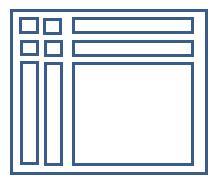
\includegraphics[width=5cm]{./figures/PTCont1.pdf}
\caption{$\mat H'$ 矩阵的结构} 
\end{figure}

方格子代表 $C_{ij} = \bra{i} H' \ket{j}$, 横条代表 $H_{\I\bvec k'} = \mel{i}{H'}{k'}$,  纵条代表 $H_{\bvec k j} = \mel{\bvec k}{H'}{j}$. 

与离散的情况相似, 微扰理论的推导方法是先把 $\ket{\psi}$ 代入含时薛定谔方程, 然后两边分别左乘基底 $\bra{i}$ 和 $\bra{\bvec k}$,  注意后者这里要使用动量归一化条件把对 $\bvec k$ 的积分消去. 微扰递推公式为
 \begin{equation}
C_i^{(n + 1)}(t) = \frac{1}{\I\hbar} \int \dd{t'} \qty(\sum_{j \ne i} H'_{ij} C_j^{(n)} + \int H_{\I\bvec k'} \phi ^{(n)} (\bvec k') \dd[3]{k'} )
\end{equation}
\begin{equation}
\phi^{(n+1)}(\bvec k) = \frac{1}{\I\hbar} \int \dd{t'} \qty(\sum_j H'_{\bvec kj} C_j^{(n)} + \int H_{\bvec k\bvec k'} \phi ^{(n)}(\bvec k') \dd[3]{k'})
\end{equation}
关于 $\ket{\bvec k}$  的定义, 若势能函数是局部的, 那么在无穷远处波函数是平面波, 由此来定义 $\bvec k$.  这样, 在计算 $\braket{\bvec k'}{\bvec k}$ 时, 由于积分范围是无穷, 可以忽略局部势能对波函数的影响, 所以归一化系数就是 $\E^{\I \bvec k\bvec r} = \E^{\I k_x x} \E^{\I k_y y} \E^{\I k_z z}$ 的归一化系数即 $1/{(2\pi )^{3/2}}$. 
 
